\section{Topological Walk on Spheres}
\label{sec:method}

Equation~\eqref{eq:localproduct} turns a domain-perturbation limit into two point queries on the original domain.  This section constructs an estimator that remains correct under the correlated reuse patterns needed in a fast implementation.

\subsection{Primal and adjoint random-walk oracles}

At candidate $z$, let a WoS/WoSt implementation return a random pair
\begin{equation}
  X_i(z):=(U_i(z),P_i(z)), \qquad i=1,\dots,N,
\end{equation}
where pairs are independent and identically distributed across $i$, but $U_i$ and $P_i$ may share a seed, geometric queries, path prefixes, or a harmonic cache.  We first analyze exact oracles,
\begin{equation}
  \E[U_i(z)]=u(z),\qquad \E[P_i(z)]=p(z),
  \label{eq:oraclemeans}
\end{equation}
and later place termination and cache error into an explicit bias budget.  Screened Poisson killing, source sampling, Walk on Stars, and variance reduction can all live behind this interface.

\paragraph{The independence unit is an entire randomization.}
For Array-RQMC or a randomly constructed cache shared across many trajectories,
individual paths are not independent oracle pairs.  Instead, generate $R\ge2$
independent complete randomizations and use their field averages
$X_r=(\bar U_r,\bar P_r)$ in \cref{eq:ustatpairwise}, with $N=R$.
Within a randomization, primal and adjoint may reuse every trajectory; neighbor
queries may also share all cached paths.  Different randomizations must use
independent random streams and independently generated random caches.
The finite-sample radius then uses $\lfloor R/2\rfloor$, not the number of
paths or cross-products.  This interface preserves compatibility with
Array-RQMC~\cite{ho2026array} and neighbor reuse~\cite{czekanski2026neighbors}
without importing an independence assumption they do not satisfy.
The exact bias identities and a counterexample appear in
\cref{app:batchindependence}.

The source-integral identity used by our three-dimensional Poisson implementation is stated and proved in \cref{prop:greenballsample}. General objectives require a valid adjoint oracle as well as a state oracle; the product construction does not by itself solve the adjoint PDE or remove bias from a learned or approximate adjoint source. Compliance experiments exploit $p=u$; sensor-protection experiments solve the distinct adjoint driven by the observation weight.

A naive product from a same-seed pair is biased whenever $U_i$ and $P_i$ are correlated; its bias is $-\Cov(U_i,P_i)$.  Independently generating every primal and adjoint path avoids that covariance but forfeits useful reuse.  We instead remove all same-index products.

\begin{figure}[t]
 \centering
 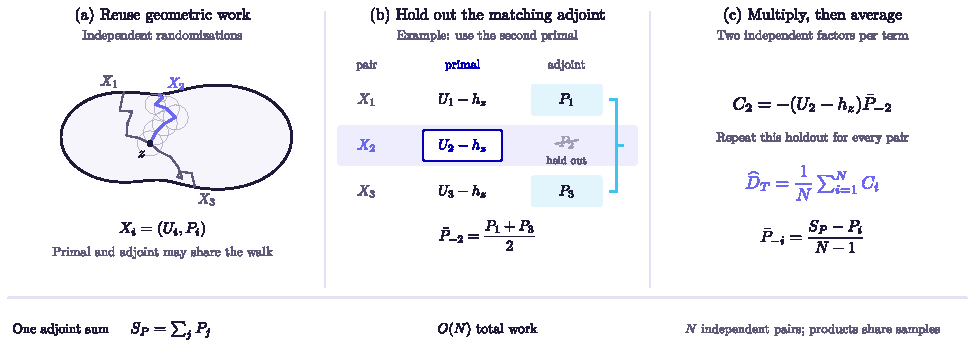
\includegraphics[width=\textwidth]{figures/crossfit.pdf}
 \caption{\textbf{A leave-one-out view of the cross-fitted estimator.} (a) Independent randomizations produce pairs $X_i=(U_i,P_i)$; both components may reuse the same walk geometry. (b) For the example $i=2$, retain $U_2-h_z$ and average the other adjoints, excluding the potentially correlated $P_2$. (c) Form $C_i=-(U_i-h_z)\bar P_{-i}$ and average over $i$. Each product has independent factors; the products themselves share samples. One adjoint sum evaluates every leave-one-out mean in $O(N)$ total work. This is exactly the estimator in \cref{eq:ustatpairwise}; unbiasedness requires unbiased marginal oracles. Walks are schematic.}
 \label{fig:crossfit}
\end{figure}

\subsection{Cross-fitted product estimator}

Define
\begin{align}
 \widehat{\DT}_N(z)
 &:=-\frac{1}{N(N-1)}
    \sum_{i\ne j}\bigl(U_i(z)-h_z\bigr)P_j(z) 
    \label{eq:ustatpairwise}\\
 &=-\frac{
   \bigl(\sum_i(U_i-h_z)\bigr)\bigl(\sum_iP_i\bigr)
   -\sum_i(U_i-h_z)P_i}
  {N(N-1)}.
  \label{eq:ustatlinear}
\end{align}
The second form costs $O(N)$ rather than $O(N^2)$.  It is a symmetric, order-two U-statistic~\cite{hoeffding1948class} with kernel
\begin{equation}
 H(X_i,X_j):=-\tfrac12\left[(U_i-h_z)P_j+(U_j-h_z)P_i\right].
 \label{eq:kernel}
\end{equation}
The factors in every cross-index product are independent, so arbitrary dependence inside $X_i$ is harmless. \Cref{thm:unbiased,thm:variance} formalize this observation. Equivalently, \cref{fig:crossfit} keeps $U_i-h_z$, pairs it with the leave-one-out mean $\bar P_{-i}=(\sum_jP_j-P_i)/(N-1)$, and averages over $i$. Only the matching $P_i$, which may share randomness with $U_i$, is omitted from that term.

\subsection{One set of paths, many candidate sites}

The algebra above is pointwise, but the optimizer must evaluate thousands of $z$ values.  The estimator permits two complementary reuse modes; our main 3D design studies use pointwise scouting, and the separate accelerated-sampling study evaluates selected reuse mechanisms:

\begin{enumerate}
  \item \textbf{Unbiased scout.}  Boundary-value caching or stochastically truncated harmonic caching turns each completed walk into a local expansion that can be queried at multiple candidates without changing its expectation~\cite{miller2023boundary,zhou2025harmonic}.  We retain the independent cache index $i$ required by \cref{eq:ustatpairwise}.
  \item \textbf{Approximate scout, bias-controlled validation.}  A low-order deterministic cache or self-normalized probe estimator may be much faster but slightly biased~\cite{huang2026probe}.  It may rank sites, but it never certifies insertion.  The selected sites are re-evaluated with fresh unbiased paths; alternatively, a proven cache bias $b_{\mathrm{cache}}$ is included in \cref{eq:certificate}.
\end{enumerate}

This separation is important.  Reusing samples after adaptively choosing the most negative noisy location produces a winner's-curse bias even when every pointwise estimator is unbiased.  For a preselected site, fresh validation avoids reusing its selection noise. Choosing again among several freshly rescored sites requires simultaneous coverage, or another independent final check, to support a certificate.

\subsection{Estimator interface}

A certifying implementation must supply the tuple
\begin{equation}
 (\widehat{\DT}_N,\ r_N(\delta),\ b_{\mathrm{term}},\ b_{\mathrm{cache}}),
 \label{eq:estimatorinterface}
\end{equation}
where $r_N$ is a statistical confidence radius and the two $b$ terms upper-bound deterministic or algorithmic bias.  The optimizer is agnostic to whether $r_N$ comes from the bounded-sample result in \cref{thm:concentration}, an empirical-Bernstein construction, or a robust median-of-means variant.  It only requires a valid coverage statement.
